In this chapter, we return to a controller that prevents a vehicle from
violating a boundary in one spatial dimension. Controllers with this
objective were described in Chapters~\ref{chap:memo15}
and~\ref{chap:emsoft16}. However, as described in Section~\ref{sec:flight}
of Chapter~\ref{chap:emsoft16}, those controllers exhibit significant
oscillation near the boundary due to a discontinuity in the value output by
the controllers. This oscillation is undesirable from the perspective of
the pilot. More significantly, it is physically impossible to change
control signal discontinuously, so the actual implementation deviates from
the model at the boundary, partially causing the boundary violations that
we experienced in actual flight tests.

Our goal was to build a controller whose behavior at the boundaries was
acceptable for the popular open source UAV autopilot called
Ardupilot~\cite{ardupilot}. We worked with Ardupilot developers to build
such a controller as a component of their new geofence module, which
prevents vehicle from exiting a specified safe zone, regardless of what the
pilot does. Crucially the controller that we built did not have a
discontinuity at the boundary, and flight tests confirmed that this
eliminated violations. After building the controller, we attempted to
verify safety of a model of the controller in one spatial dimension.
However, while attempting this task, we found several important gaps in
existing work on formal verification of cyber-physical systems. In this
chapter, we present several proof rules and techniques that address these
shortcomings, and apply them to verify a double integrator model of the
Ardupilot controller in one spatial dimension.

First, deductive techniques for hybrid systems typically involve some
continuous analogue of induction, such as differential
induction~\cite{Platzer10DAL}, whose mechanical verification we
discussed in Chapter~\ref{chap:memo15}, or barrier
certificates~\cite{prajna04barrier}. These techniques provide conditions
for verifying that a state predicate is an invariant of a system of
differential equations, without actually solving the system of
equations. However, differential induction and the original formulation of
barrier certificates from~\cite{prajna04barrier} are too weak to verify
invariants for certain systems, particularly those whose solutions
exponentially decay towards the invariant boundary. For example, these
techniques cannot verify invariance of $y \leq 0$ along solutions of the
system $\dt{y} = -y$. Systems of this form arise naturally when building a
controller like the one designed for Ardupilot -- the controller should
allow the vehicle to approach the boundary and smoothly come to a stop at
the boundary. In order to verify this, differential induction must be
augmented with another proof rule called differential
auxiliaries~\cite{Platzer12diffcut}.

On the other hand, recent work from the control theory
community~\cite{kong2013barrier,xu15barrier,nguyen16barrier} has produced a
new version of barrier certificates that is less conservative than prior
work. In particular, the condition required for invariance captures
exponential decay towards the invariant boundary. We provide the first
implementation of this approach in a formal verification context, and
demonstrate its ease of use on the controller that we designed for
Ardupilot.

Second, control systems are often designed under the assumption that
controllers run continuously, while the actual implementation is a
sampled-data system, the topic of this disseration. That is, the digitial
controller runs periodically rather than continuously. System designers can
compensate for this (and other) approximations by adding a safety
``buffer'' to the system. For example, the Ardupilot controller we helped
build stops the vehicle 1 meter prior to the actual safety boundary. In
order to reason about whether such a buffer is sufficient for a given
system, we augmented the new barrier certificate proof rule
from~\cite{kong2013barrier,xu15barrier,nguyen16barrier} to bound the error
introduced by a continuous time approximation of a sampled-data
system. This rule allows one to perform the majority of reasoning in a
purely continuous model using powerful techniques resulting from over a
century of control theory research. We use this rule to show that the
constant sized buffer is, in fact, sufficient to compensate for the
continuous time approximation of the Ardupilot controller.

Finally, other formal verification frameworks are unable to apply
differential induction and barrier certificates to invariants involving
piecewise functions.  We show how to remove this restriction by working in
the expressive Coq proof assistant. This allows us to verify the critical
piecewise invariant arising in the Ardupilot controller.

\section{Overview}
\label{sec:exp-smpl-overview}
Ardupilot is a popular open source autopilot installed in over 1,000,000
vehicles, including quadcopters and other UAVs~\cite{ardupilot}. The
geofence module allows one to specify a 2D polygon safe region. The pilot
is free to move arbitrarily within the polygon, but the module restricts
movement near the boundary and ultimately stops the vehicle within 1 meter
of the boundary.

We focus on the controller logic for stopping the vehicle 1 meter before
the boundary in one spatial dimension. This logic must satisfy three
criteria: (1) allow unrestricted movement when the vehicle is far from the
boundary, (2) take into account limitations on maximum possible braking
force of the system, and (3) bring the vehicle smoothly to a stop at the 1
meter buffer.

The module does so by restricting the velocity as a function of the
vehicle's distance from the boundary. Given the maximum braking force of
the systems, a natural approach is to limit the velocity as a function of
the \emph{square root} of the distance from the boundary. However, such a
limitation results in a discontinuity in control at the boundary, as
experienced by the controllers in Chapters~\ref{chap:memo15}
and~\ref{chap:emsoft16}. In control theory terminology, such a system
behaves as a bang-bang controller, which allows maximum positive
acceleration until the last possible moment, when maximum braking force is
applied. Such controllers suffer from oscillations at the boundary,
violating the third criteria (smoothness).

A solution developed by the Ardupilot engineers is to apply a piecewise
limitation to velocity -- far from the boundary enforce a square root
relationship between position and velocity, while close to the boundary,
enforce a linear relationship. Such a linear relationship removes the
control discontinuity at the boundary. Section~\ref{sec:proof-geofence}
provides the formal details of the velocity restriction.

The actual system passes the resicted velocity to an underlying velocity
controller. In this chapter, we ignore the dynamics of the inner loop
velocity controller controller and as in the rest of this dissertation,
treat the system as a double integrator, in which the control law outputs
acceleration. Such an approximation is an important first step towards
developing new formal verification techniques, as it still forces us to
handle the non-trivial velocity restriction law.  We leave composition with
the velocity controller as an interesting direction for future work.

Given the double integrator model and the velocity restriction law, we show
how to derive the controller's logic to guarantee the velocity restriction
and thus enforce the boundary on position. This logic comes in the form of
state-dependent upper bounds on the control signal (acceleration). The
actual control law implementation takes the minimum of these constraints
and the pilot's desired acceleration. Crucially, we derive these
constraints using our barrier certificate theorem for sampled-data systems,
which allows us to derive the constraints assuming a continuous controller,
and transfer these results to the sampled-data model by proving two simple
side-conditions on the intersample system behavior.

Section~\ref{sec:model} presents the formal logic we use to reason about
sampled-data systems and gives a double integrator model of the geofence
within this logic. Section~\ref{sec:proof} provides formal details on
barrier certificates for sampled-data systems and shows how to apply them
to reason about the geofence. Section~\ref{sec:coq} describes the Coq
implementation of our results with Section~\ref{sec:differentiation}
describing how we extend formal verification using barrier certificate to
piecewise functions.

\section{Logic}
\label{sec:model}
This chapter uses a different formal framework than the previous
chapters. Rather than linear temporal logic, we use a logic over system
trajectories, i.e. functions $\trajectory{n}$ from time to state.

Our logic is defined in terms of two relations: models (written $F \models
P$) expresses that a trajectory predicate $P$ holds on a trajectory $F$;
and entails (written $P \entails Q$) expresses that a trajectory predicate
$Q$ holds on all trajectories that $P$ holds on.

Formally, entailment is defined as follows:
\begin{definition}[Entailment]
For trajectory predicates $P$ and $Q$,
\[
P \entails Q \defeq \forall F \in \trajectory{n} : F \models P \implies F \models Q
\]
\label{def:entailment}
\end{definition}

We now define the models relation for several types of predicates. First,
we define models for a predicate that expresses whether a trajectory is a
valid solution to a sampled-data system whose intersample dynamics are
given by $\dt{\vecbold{z}} = f(\vecbold{z},u(\vecbold{z_k}))$ where
$\vecbold{z_k}$ is the state at the last sample and $u \in \R^n \rightarrow
\R^m$ is the control law. This definition requires a notion of well-formed
sample times:
\begin{definition}[Sample times]
A sampling sequence $t_k$ with $k \in \N$ is well-formed with bound $\Delta$ if
\[\begin{array}{lr}
t_0 = 0 & \wedge \\
\forall k \in \N : 0 < t_{k + 1} - t_k \leq \Delta & \wedge \\
\forall t \in \Rpos : \exists k \in \N : t_k \leq t < t_{k + 1}
\end{array}
\]
\end{definition}
Using the definition of well-formed sample times, we can formally specify
the models relation for a sampled-data system whose sample times (time
between discrete controller executions is bounded by $\Delta$:
\begin{definition}[Sampled data solutions]
\begin{align*}
F \models \evolvessmpl{\dt{\vecbold{z}} = f(\vecbold{z},u)}{\Delta}
\defeq&~\exists t_k \in \{ t_k : t_k \text{ well-formed} \} : \\
&\qquad \forall k \in \N : \forall t \in [t_k,t_{k+1}) : \dt{F}(t) = f(F(t),u(F(t_k)))
\end{align*}
\label{def:solution-smpl}
\end{definition}
In Definition~\ref{def:solution-smpl}, we enforce more structure on the
system than our \SysA{} abstraction from previous chapters
(Definition~\ref{def:sys-abstraction}). In particular, we make explicit the
control law and enforce that the control input is held constant between
samples. Adding this structure allows us to state a powerful barrier
function theorem for sampled-data systems.

Definition~\ref{def:solution-smpl} does not put any restrictions on the
initial state of the trajectory, $F(0)$. For this, we use state
predicates -- predicates over a single state. A state predicate holds on
a trajectory if it holds on the initial state of that trajectory:
\begin{definition}[Initially]
For a state predicate $P$ and a trajectory $F$,
\[
F \models P \defeq F(0) \models P
\]
\label{def:init}
\end{definition}

Next, we need to express that a state predicate is an invariant of a
trajectory. For this, we define an always operator, which takes a state
predicate and expresses that it holds for all time along a trajectory.
\begin{definition}[Always]
For a state predicate $P$ and a trajectory $F$,
\[
F \models \Always{P} \defeq \forall t \in \Rnneg : F(t) \models P
\]
\label{def:always}
\end{definition}

Finally, sampled-data systems often have an upper bound on the time between
samples. Thus, we define a bounded always operator in order to reason about
invariants between samples. This operator takes a state predicate and
expresses that it holds until a time bound $\Delta$ along a trajectory.
\begin{definition}[Bounded Always]
For a state predicate $P$, a constant $\Delta \in \Rnneg$, and a trajectory $F$,
\[
F \models \AlwaysT{\Delta}{P} \defeq \forall 0 \leq t \leq \Delta : F(t) \models P
\]
\label{def:bounded-always}
\end{definition}

\section{Exponential barrier certificates}
\label{sec:proof-barrier}
Deductive approaches to hybrid system verification typically involve a
continuous analogue of induction. Barrier certificates are one such
technique. In the typical formulation of barrier certificates, one proves
the invariance of $B(\vecbold{z}) \leq 0$ by proving that the value of
$B(\vecbold{z})$ does not increase along trajectories of the system. Recent
work from control theory~\cite{kong2013barrier} has relaxed this
requirement -- the rate of change of $B(\vecbold{z})$ along trajectories
must be proportional to its value. This allows the value of
$B(\vecbold{z})$ to increase along trajectories, but requires that the rate
of change slow as trajectories approach the boundary $B(\vecbold{z}) =
0$. Essentially, $B(\vecbold{z})$ can exponentially decay towards the
boundary but never cross it.

In this section, we present two barrier certificate proof rules for
sampled-data systems.  The first (Lemma~\ref{thm:barrier-smpl-weak}) is a
trivial adaptation of the rule from~\cite{kong2013barrier} to sampled-data
systems. We explain why this rule, by itself, is insufficient.  Then we
present our new version of exponential barrier certificates for
sampled-data systems that decomposes verification into an exponential decay
property of the continuous time system approximation and two simple
properties about the intersample behavior
(Theorem~\ref{thm:barrier-smpl}). In Section~\ref{sec:proof-geofence}, we
show how to use these proof rules to reason about the Ardupilot
controller. All results in this section have been formalized in the Coq
proof assistant. To the best of our knowledge, this is the first such
formalization of exponential barrier certificates.

Barrier certificates are functions $B \in \R^n \rightarrow \R$ that assign
a scalar to every state. One establishes the invariance of $B(\vecbold{z})
\leq 0$ by proving a property about the rate of change of $B(\vecbold{z})$
along trajectories of the system. Formally, $\nabla B \dotprod
f(\vecbold{z},\vecbold{z_k})$ gives the rate of change or time derivative
of $B$ along trajectories of the system, also known as the Lie derivative
of $B$. Here, $\nabla B$ denotes the gradient of $B$, or vector of partial
derivatives $[\frac{\partial B}{\partial x_1},\ldots,\frac{\partial
    B}{\partial x_n}]$.

Lemma~\ref{thm:barrier-smpl-weak} gives our trivial adaptation of barrier
certificates from~\cite{kong2013barrier} to sampled-data systems.

\begin{lemma}
Consider a continuously differentiable function $B \in \R^n \rightarrow
\R$, constants $\lambda \in \R$ and $\Delta \in \Rpos$, and a state
predicate $P$. If the following condition holds:
\[
\forall \vecbold{z}, \vecbold{z_k} \in \{\vecbold{y} \in \R^n~|~\vecbold{y} \models P\} : \nabla B \dotprod f(\vecbold{z},\vecbold{z_k}) \leq \lambda B(\vecbold{z})
\]
then
\[
\begin{array}{cl}
&
B(\vecbold{z}) \leq 0~\wedge~
\Always{P}~\wedge~
\evolvessmpl{\dt{\vecbold{z}} = f(\vecbold{z},u(\vecbold{z_k}))}{\Delta} \\
\entails
&
\Always{B(\vecbold{z}) \leq 0}
\end{array}
\]
\label{thm:barrier-smpl-weak}
\end{lemma}
% TODO: Can we claim novelty here by putting P into the theorem. This is
% essentially a combination of differential cut and the exponential
% condition, but doesn't seem to have been stated together anywhere.

Lemma~\ref{thm:barrier-smpl-weak} states that if $B(\vecbold{z}) \leq 0$
holds initially, and if, assuming a known invariant $P$, the time
derivative of $B$ is at most proportional to its value, then
$B(\vecbold{z}) \leq 0$ is an invariant.

While this theorem is powerful for continuous time systems, it is lacking
for sampled-data systems. The problem is that the premise of the theorem
does not constrain the relationship between the sampled state
$\vecbold{z_k}$ and the current state $\vecbold{z}$. However, as we will
see, this theorem still has utility. In particular, once an invariant $P$
has been established using Theorem~\ref{thm:barrier-smpl},
Lemma~\ref{thm:barrier-smpl-weak} can be used to establish a new invariant
using the invariance of $P$.

We would like the premise of Theorem~\ref{thm:barrier-smpl-weak} to be
relaxed so that the control input $u$ is applied continuously. In other
words, we would like to only prove $\nabla B \dotprod
f(\vecbold{z},\vecbold{z}) \leq \lambda B(\vecbold{z})$ rather than $\nabla
B \dotprod f(\vecbold{z},\vecbold{z_k}) \leq \lambda B(\vecbold{z})$. We
can achieve this relaxation if we can establish an additional condition on
the intersample behavior: the time derivative of $B$ does not change by
more than a constant $C$ between samples. Under such a condition, the
property $B(\vecbold{z}) \leq 0$ is not an invariant, but $B(\vecbold{z})
\leq C\cdot \Delta$ is. This mirrors a control design practice -- treat the
controller as continuous and add a constant safety buffer to account for
the approximation error.

This argument is formalized in
Theorem~\ref{thm:barrier-smpl}. Condition~\eqref{thm:barrier-smpl-exp} is
the relaxed version of the premise of
Theorem~\ref{thm:barrier-smpl-weak}. Condition~\eqref{thm:barrier-smpl-inter}
characterizes the behavior of the state between samples, while
condition~\eqref{thm:barrier-smpl-deriv-change} bounds the change in time
derivative of $B$, under the characterization established
by~\eqref{thm:barrier-smpl-inter}. Such a decomposition allows us to use
any continuous reasoning technique to
dispatch~\eqref{thm:barrier-smpl-inter} and arithmetic reasoning to
establish~\eqref{thm:barrier-smpl-deriv-change}.

\begin{theorem}
Consider a continuously differentiable function $B \in \R^n \rightarrow
\R$, constants $C,\Delta \in \Rpos$, a state predicate $P$, and a state
relation $S$. If the following conditions hold:
\begin{enumerate}[label=\roman*), ref=\roman*]
\item
\label{thm:barrier-smpl-exp}
$\forall \vecbold{z} \in \{\vecbold{y} \in \R^n~|~\vecbold{y} \models P\} : \nabla B \dotprod f(\vecbold{z},\vecbold{z}) \leq -\frac{B(\vecbold{z})}{\Delta}$
\item
\label{thm:barrier-smpl-inter}
$\forall \vecbold{z_k} \in \R^n : \vecbold{z} = \vecbold{z_k} \wedge \evolvessmpl{\dt{\vecbold{z}} = f(\vecbold{z},\vecbold{z_k})}{\Delta} \entails \AlwaysT{\Delta}{(\vecbold{z}_k,\vecbold{z}) \in S}$
\item
\label{thm:barrier-smpl-deriv-change}
$\forall (\vecbold{z_k}, \vecbold{z}) \in S : \nabla B \dotprod f(\vecbold{z},\vecbold{z_k}) \leq \max{(\nabla B \dotprod f(\vecbold{z_k},\vecbold{z_k}) + C,0)}$
\end{enumerate}
then
\[
\begin{array}{cl}
&
B(\vecbold{z}) \leq C \cdot \Delta~\wedge~
\Always{P}~\wedge~
\evolvessmpl{\dt{\vecbold{z}} = f(\vecbold{z},u(\vecbold{z_k}))}{\Delta} \\
\entails
&
\Always{B(\vecbold{z}) \leq C \cdot \Delta}
\end{array}
\]
\label{thm:barrier-smpl}
\end{theorem}
%TODO dB must be continuous
\begin{proof}
For any $k$ and for any $t \in [t_k, t_{k+1})$,
\begin{align}
\nonumber
B(\vecbold{z}(t)) - B(\vecbold{z}(t_k)) &= \int_{t_k}^t \nabla B \dotprod f(\vecbold{z}(\tau),\vecbold{z}(t_k)) d\tau\\
\tag{by~\eqref{thm:barrier-smpl-deriv-change} and~\eqref{thm:barrier-smpl-inter}}
&\leq \int_{t_k}^t \big(\max{(\nabla B \dotprod f(\vecbold{z}(t_k),\vecbold{z}(t_k)) + C,0)}\big) d\tau \\
\tag{by~\eqref{thm:barrier-smpl-exp}}
&\leq \int_{t_k}^t \left(\max({-\frac{B(\vecbold{z}(t_k))}{\Delta} + C,0)}\right) d\tau \\
\nonumber
&= (t - t_k) \cdot \left(\max{(-\frac{B(\vecbold{z}(t_k))}{\Delta} + C,0)}\right)
\end{align}

Therefore, for any $k$ and any $t \in [t_k,t_{k+1})$, since $t - t_k \leq Delta$,
\begin{equation}
B(\vecbold{z}(t_k)) \leq C\cdot \Delta \implies B(\vecbold{z}(t)) \leq C\cdot \Delta
\end{equation}
By induction on $k$, $\forall t \geq 0 : B(\vecbold{z}(t)) \leq C\cdot \Delta$
\end{proof}

Note the $\max{}$ in condition~\eqref{thm:barrier-smpl-deriv-change} of
Theorem~\ref{thm:barrier-smpl}. The intersample derivative of $B$ does not
need to be close to the sample time derivative of $B$ as long as it is
non-positive. This subtlety bares a resemblance to the normal formulation
of barrier certificates in which the time derivative of $B$ must always be
non-positive.

\section{Ardupilot controller}
\label{sec:proof-geofence}
Now that we have established the general theory, we can use it to reason
about a double integrator model of the Ardupilot controller, whose
intersample behavior is given by:
\[
\dt{x} = v, \dt{v} = u(x_k,v_k)
\]
The control law $u$ is designed to enforce $x \leq 0$.  We begin this
section by describing how $u$ is designed to (almost) achieve this
objective. As mentioned in Section~\ref{sec:exp-smpl-overview}, the control
law design comes in the form of state-dependent upper bounds on the control
signal $u$. As described in that section, the actual control law
implementation takes the minimum of the pilot's desired acceleration and
those constraints.

The Ardupilot control law was designed assuming that the law is applied
continuously (not as a sampled-data system). This approximation simplifies
design and reasoning but also introduces an error, which actually results
in a violation of $x \leq 0$. We will ultimately apply
Theorem~\ref{thm:barrier-smpl} to quantify this violation.

Relevant to the controller design are the physical constraints on the
system, particularly the maximum possible acceleration. Since we are
interested in a controller that stops the system's position from violating
some boundary, the important physical constraint is a limit on the system's
braking acceleration. That is, we need to ensure that the control law does
not require deceleration of a greater magnitude than is physically
possible. We denote by $\umax$ this magnitude -- we need to ensure that the
system never reaches a state $x,v$ in which $u(x,v) < -\umax$.

Since the stopping distance for a particle with acceleration $a$ and
initial velocity $v$ is $\frac{v^2}{2a}$, the $\umax$ constraint implies
that the system must enforce the following invariant:
\[
x \leq \frac{\max{(v,0)}^2}{2\umax}
\]
However, since the controller was designed under a continuous time
approximation, the invariant needs to be strengthened by using a more
conservative braking acceleration $\umaxc < \umax$. At the end of this
section, we will give precise conditions on $\umaxc$ to ensure that the
system never reaches a state $x,v$ in which $u(x,v) < -\umax$. The
strengthened invariant is thus:
\[
x \leq \frac{\max{(v,0)}^2}{2\umaxc}
\]
This invariant is still insufficient. The problem is that such an invariant
will result in a control discontinuity at the position boundary $x =
0$. This occurs if the system is in a state in which $x =
\frac{\max{(v,0)}^2}{2\umaxc}$. Such a state requires that the controller
issue constant acceleration $-\umaxc < 0$ when $x < 0$ and permits zero
acceleration when $x = 0$. As described in the introduction, such a control
law produces undesirable oscillations at the boundary and is physically
impossible.

To solve this problem, the Ardupilot developers designed a more
conservative invariant that is a piecewise function of the distance from
the boundary. Close to the boundary, the velocity limit is linear in the
distance, while farther away, the velocity limit is proportional to the
square root of the distance. This relationship is depicted in
Figure~\ref{fig:sqrt-lin}. Notice that the piecewise transition between
these two relationships occurs where they are tangent. This ensures that
(a) a barrier certificate describing the region is continuously
differentiable, and (b) the control constraints induced by such a barrier
are continuous.

\begin{figure}
\centering
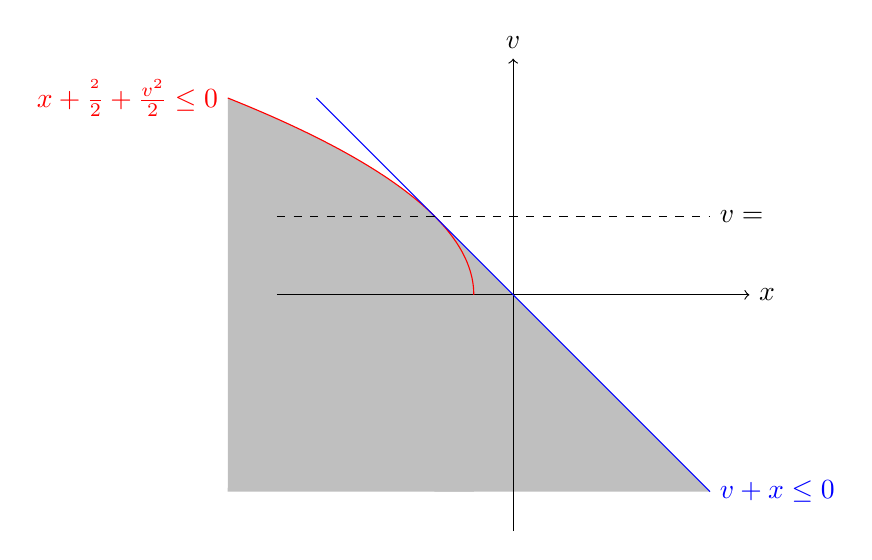
\begin{tikzpicture}
      \fill [lightgray, domain=0:2.5, variable=\x]
        (-0.5,-2.5)
        -- plot ({-\x*\x/2 - 1/2}, {\x})
        -- (-3.625, -2.5)
        -- cycle;
      \fill [lightgray, domain=-1:2.5, variable=\x]
        (-1, -2.5)
        -- plot ({\x}, {-\x})
        -- cycle;
      \draw[->] (-3,0) -- (3,0) node[right] {$x$};
      \draw[->] (0,-3) -- (0,3) node[above] {$v$};
      \draw[domain=0:2.5,smooth,variable=\v,red]  plot ({-\v*\v/2 - 1/2},{\v})
          node[left] at (-3.625,2.5) {$x + \frac{\umaxc \p^2}{2} + \frac{v^2}{2\umaxc} \leq 0$};
      \draw[domain=-2.5:2.5,smooth,variable=\x,blue]  plot ({\x},{-\x}) node[right] at (2.5,-2.5) {$\p v + x \leq 0$};
      \draw[black,variable=\x,domain=-3:2.5,dashed] plot ({\x},{1}) node[right] at (2.5,1) {$v = \umaxc \p$};
\end{tikzpicture}
\caption{A depiction of $\Bpw (x,v) \leq 0$ where the red curve represents the first branch of the piecewise function and blue the second.}
\label{fig:sqrt-lin}
\end{figure}

Formally, the region depicted in Figure~\ref{fig:sqrt-lin} is $\Bpw (x,v)
\leq 0$, where
\begin{equation}
\Bpw (x,v) =
\begin{cases}
\p v + x & \text{if } v \leq \umaxc\p \\
x + \frac{\umaxc \p^2}{2} + \frac{v^2}{2\umaxc} & \text{otherwise}
\end{cases}
\label{eq:barrier-piecewise-dbl-int}
\end{equation}
Our goal is to (almost) enforce the invariance of $x \leq 0$ -- that is, we
would like to enforce $x \leq K$ for some positive constant $K$.  We now
take a two step process to prove the invariance of $x \leq K$ for some
constant $K$. First, we use Theorem~\ref{thm:barrier-smpl} and constraints
on $u$ to prove the invariance of $\Bpw (x,v) \leq K$. Then we use
Lemma~\ref{thm:barrier-smpl-weak} and the invariance of $\Bpw (x,v) \leq K$
to prove the invariance of $x \leq K$. The assumptions on $u$ are as
follows:
\begin{assumption}
For any $x,v \in \R$,
\[
u(x,v) \leq
\begin{cases}
\frac{-(\p v + x)}{T\p} - \frac{v}{\p} & \text{if } v \leq \umaxc\p \\
\frac{-\umaxc x}{T v} - \frac{\umaxc^2 \p^2}{2Tv} - \frac{v}{2T} - \umaxc & \text{otherwise}
\end{cases}
\]
\label{ass:u_pw_bound}
\end{assumption}

Note that the division by $v$ in the second branch of
assumption~\ref{ass:u_pw_bound} is not problematic, since in that branch,
$v > \umaxc\p > 0$.

Since the control law was designed using a continuous time approximation,
we need to put a constant upper bound on the control in order to bound the
intersample behavior and thus apply Theorem~\ref{thm:barrier-smpl}. Such a
bound is captured in the following assumption:
\begin{assumption}
$\forall x, v \in \R : u(x,v) \leq \umaxc$
\label{ass:u_umax_bound}
\end{assumption}

Theorem~\ref{thm:barrier-smpl} requires reasoning about the time derivative
of $\Bpw$, which is given by~\eqref{eq:dbarrier-piecewise-dbl-int}. The
formal details details of reasoning about Lie derivatives of piecewise
functions, like the one in~\eqref{eq:dbarrier-piecewise-dbl-int} are
deferred to Section~\ref{sec:differentiation}.
%TODO explain why we quantify over v and v_k but not x and x_k
\begin{equation}
\forall v, x_k, v_k \in \R : \nabla \Bpw \dotprod [v,u(x_k,v_k)] =
\begin{cases}
\p u(x_k,v_k) + v & \text{if } v \leq \umaxc\p \\
v + \frac{v\cdot u(x_k,v_k)}{\umaxc} & \text{otherwise}
\end{cases}
\label{eq:dbarrier-piecewise-dbl-int}
\end{equation}

The next three lemmas satisfy the three conditions of
Theorem~\ref{thm:barrier-smpl} for $\Bpw$.

\begin{lemma}[Condition~\eqref{thm:barrier-smpl-exp}]
For any $x,v \in \R$,
\[
\nabla \Bpw \dotprod [v,u(x,v)] \leq -\frac{\Bpw (x,v)}{\Delta}
\]
\label{lem:exp-condition-dbl-int}
\end{lemma}
\begin{proof}
Solving the above in equality for $u$ results in exactly the inequality in
assumption~\ref{ass:u_pw_bound}.
\end{proof}

\begin{lemma}[Condition~\eqref{thm:barrier-smpl-inter}]
For any $x_k, v_k \in \R$,
\[
\begin{array}{cl}
& x = x_k~\wedge~v=v_k~\wedge~\evolvessmpl{\dt{x}=v,\dt{v}=u(x_k,v_k)}{\Delta} \\
\entails
& \AlwaysT{\Delta}{v \leq v_k + \max{(u(x_k,v_k), 0)}\cdot \Delta}
\end{array}
\]
\label{lem:intersmpl-dbl-int}
\end{lemma}
\begin{proof}
By integration of $v$ from 0 to $\Delta$.
\end{proof}

The intersample dynamics are sufficiently simple that
Lemma~\ref{lem:intersmpl-dbl-int} can be proven by integration. However,
since condition~\eqref{thm:barrier-smpl-inter} of
Theorem~\ref{thm:barrier-smpl} concerns purely continuous time dynamics,
the intersample behavior of more complex systems can be verified using a
number of powerful techniques from prior work, including differential
induction~\cite{Platzer10DAL}. Making such a connection formal is an
interesting direction for future work.

\begin{lemma}[Condition~\eqref{thm:barrier-smpl-deriv-change}]
For any $x_k, x, v_k, v \in \R$ such that $v \leq v_k + \max{(u(x_k,v_k),
  0)}\cdot \Delta$,
\[
\nabla \Bpw \dotprod [v,u(x_k,v_k)] \leq \nabla \Bpw \dotprod [v_k,u(x_k,v_k)] + \violation
\]
\label{lem:deriv-change-dbl-int}
\end{lemma}
\begin{proof}
By assumption~\ref{ass:u_umax_bound} and first order reasoning over real
arithmetic.
\end{proof}

It is important to note that the above theorem only relies on the very
simple intersample behavior of $v$ and constant bounds on $u$. It does not
rely on bounds on position nor does it depend on the more complex bounds on
$u$ used in Lemma~\ref{lem:exp-condition-dbl-int}. This serves as evidence
that Theorem~\ref{thm:barrier-smpl} allows one to prove relatively simple
side conditions in order to transfer continuous time results to the
sampled-data domain.

Given Lemmas~\ref{lem:exp-condition-dbl-int},~\ref{lem:intersmpl-dbl-int},
and~\ref{lem:deriv-change-dbl-int}, we can now prove the invariance of
$\Bpw (x,v) \leq (\violation) \cdot \Delta$.

\begin{lemma}
\[
\begin{array}{clc}
&
\Bpw (x,v) \leq (\violation) \cdot \Delta & \wedge \\
& \evolvessmpl{\dt{x}(t) = v(t), \dt{v}(t) = u(x(t_k),v(t_k))}{\Delta} & \\
\entails
&
\Always{\Bpw (x,v) \leq (\violation) \cdot \Delta} &
\end{array}
\]
\label{lem:barrier-piecewise-dbl-int}
\end{lemma}
\begin{proof}
By
Theorem~\ref{thm:barrier-smpl}. Lemmas~\ref{lem:exp-condition-dbl-int},~\ref{lem:intersmpl-dbl-int},
and~\ref{lem:deriv-change-dbl-int} satisfy
conditions~\eqref{thm:barrier-smpl-exp},~\eqref{thm:barrier-smpl-inter},
and~\eqref{thm:barrier-smpl-deriv-change} of
Theorem~\ref{thm:barrier-smpl}, respectively. We instantiate the state
predicate $P$ of Theorem~\ref{thm:barrier-smpl} with the trivial predicate
\True.
\end{proof}

Finally, given the invariance of $\Bpw (x,v) \leq (\violation) \cdot \Delta$
provided by Lemma~\ref{lem:barrier-piecewise-dbl-int}, we can return to
Theorem~\ref{thm:x-bound-dbl-int}, which establishes the invariance of $x
\leq (\violation) \cdot \Delta$. We restate the theorem here for convenience:

\begin{theorem}
\[
\begin{array}{clc}
&
\Bpw (x,v) \leq (\violation) \cdot \Delta & \wedge \\
&
x \leq (\violation) \cdot \Delta & \wedge \\
&
\evolvessmpl{\dt{x} = v, \dt{v} = u(x_k,v_k)}{\Delta} & \\
\entails
&
\Always{x \leq (\violation) \cdot \Delta} &
\end{array}
\]
\label{thm:x-bound-dbl-int}
\end{theorem}
\begin{proof}
We apply Theorem~\ref{thm:barrier-smpl-weak} with barrier function
\[
\Bx (x,v) = x - (\violation)\cdot \Delta\]
constant $\frac{-1}{\p}$, and state predicate
\[
\Bpw (x,v) \leq (\violation) \cdot \Delta
\]
Simple arithmetic reasoning reveals
that for all $x,v \in \R$,
\begin{align}
\nabla \Bx \dotprod [v,\ignorearg] + \frac{\Bx (x,v)}{\p} &\leq \Bpw (x,v) - (\violation)\cdot \Delta \\
&\leq 0
\end{align}
which satifies the premise of Theorem~\ref{thm:barrier-smpl-weak}.
\end{proof}

Theorem~\ref{thm:x-bound-dbl-int} verifies the design procedure followed by
the Ardupilot engineers -- the controller can be designed assuming that it
is applied continuously and a small constant buffer can compensate for the
approximation error. Moreover, it shows that the constraints on $u$ fall
out naturally from the velocity bounds depicted in
Figure~\ref{fig:sqrt-lin} by a simple application of
Theorem~\ref{thm:barrier-smpl}.

Finally, we provide conditions on $\umaxc$ to ensure that the system never
reaches a state $x,v$ in which $u(x,v) < -\umax$. In other words, for any
$x$ and $v$ satisfying $\Bpw (x,v) \leq (\violation) \cdot \Delta$ and $x \leq
(\violation) \cdot \Delta$, we need to ensure that there exists a value
satisfying the upper bound from assumption~\ref{ass:u_pw_bound} and the
lower bound $-\umax \leq u(x,v)$. Arithmetic reasoning reveals that the
constraints are:
\begin{equation}
\umaxc \leq \frac{\umax}{1 + \frac{2\Delta}{\p}}
\end{equation}
For Ardupilot, the sample time is small relative to $\p$, so $\umaxc$ is
close to $\umax$. This again verifies the design procedure followed by the
Ardupilot engineers -- to account for error, the controller is designed
with a conservative braking acceleration $\umaxc$ rather than the actual
physical limit $\umax$.

\section{Coq implementation}
\label{sec:coq}
We have implemented all of the results of this chapter in the Coq proof
assistant. The core theory required 571 lines of definitions and 528 lines
of proof, while the geofence model required 90 lines of definitions and 136
lines of proof. On the other hand, the Second-Derivative Controller from
Chapter~\ref{chap:emsoft16}, verified without the barrier function theorems
of this chapter, required 484 lines of proof, despite simpler constraints
on the control law. This provides evidence that
Theorem~\ref{thm:barrier-smpl} and Lemma~\ref{thm:barrier-smpl-weak} have
the potential to considerably reduce the formal proof burden for safety of
sampled-data systems.
%TODO update these numbers if proof dev changes

\subsection{Differentiation}
\label{sec:differentiation}
In Section~\ref{sec:proof}, we glossed over the formal details of verifying
the gradient of a barrier function. Working in an expressive proof
assistant like Coq allows us to verify this step as well, even for
piecewise functions. That is, we can formally prove the validity of
equations like~\eqref{eq:dbarrier-piecewise-dbl-int} using
Lemma~\ref{lem:pw-deriv}:

\begin{lemma}
For functions $e_1, e_2, e_3, e_4 \in \R^n \rightarrow \R$, variable $x$,
vector $f \in \R^n$, and constant $c \in \R$, if the following conditions
hold,
\begin{enumerate}[label=\roman*), ref=\roman*]
\item $x = c \implies e_1 = e_2$
\item $x = c \implies e_3 = e_4$
\item $x \leq c \implies \nabla e_1 \dotprod f = e_3$
\item $x \geq c \implies \nabla e_2 \dotprod f = e_4$
\end{enumerate}
then
\[
\nabla \left(
\begin{cases}
e_1 & \text{if } x \leq c \\
e_2 & \text{otherwise}
\end{cases}
\right)
\dotprod
f
=
\begin{cases}
e_3 & \text{if } x \leq c \\
e_4 & \text{otherwise}
\end{cases}
\]
\label{lem:pw-deriv}
\end{lemma}

To the best of our knowledge, this is the first formal verification
framework for hybrid systems that can handle piecewise functions.

\subsection{Logics in Coq}
%TODO should we talk about benefit of shallow encoding?
We implemented our trajectory logic using Charge!~\cite{???}, a framework
for easily defining and reasoning about logics within Coq. Charge! allows a
us to declare that a particular type forms a logic by proving that a small
set of axioms hold for that type. In our case, these axioms are proved
automatically. In return, we automatically get standard logical operators
such as conjunction, disjunction, and implication lifted into the
logic. For example, in Section~\ref{sec:proof}, we frequently wrote
formulas like $P \wedge Q$ where $P$ and $Q$ are trajectory
predicates. Without Charge!, we would have to define what it means to
conjoin two trajectory predicates. With Charge!, we get this for free.

Along with the normal logic definitions, Charge! also automatically
provides standard logical proof rules like commutativity of conjunction and
tactics to discharge simple proof obligations. In short, Charge! provides
much of the boiler-plate logical reasoning and definitions for free.

Most significantly, Charge! allows us to easily use the most appropriate
logic for each proof obligation, all within the same formal foundation of
Coq. For example, condition~\eqref{thm:barrier-smpl-inter} of
Theorem~\ref{thm:barrier-smpl} is currently phrased as a trajectory
predicate entailment. However, Platzer's differential dynamic logic
(\dL{})~\cite{Platzer15substitution} may be a better logic for reasoning
about this condition. Charge! could allow us to easily build \dL{} as a
logic in Coq and re-phrase this condition in terms of \dL{}.

%% \section{Conclusion}
%% \label{sec:conclusion}
%% The difficulty of hybrid system verification demands that we have a variety
%% of higher-order proof rules at our disposal. This work adds one such
%% powerful tool to the arsenal for the important class of sampled-data
%% systems. Moreover, we show how leveraging the expressiveness of a
%% higher-order proof assistant (Coq) allows us to extend the set of operators
%% that are in scope for formal verification using barrier certificates.

% Talk about how existing work is great for general hybrid systems, but we
% focus on writing higher order theorems that leverage the structure of
% particular classes of hybrid systems, in our case sampled-data systems.

% Do we want to talk about number of lines of proof, development effort, etc.
% Should we compare to development effort for 1D pos from emsoft paper?
% It took just a few days to verify.
